% !TeX root = vaje.tex
\chapter{Polinomi}
\label{cha:polinomi}

\section{Pregled snovi}
\label{sec:polinomi-pregled-snovi}


\subsection{Definicija polinoma}
Polinom je vsaka taka funkcija, ki jo lahko zapišemo v obliki:
\[
p(x)=a_nx^n + a_{n-1}x^{n-1}+ \cdots + a_2x^2 + a_1 x + a_0
\]
Pri tem naravno število $n$ imenujemo stopnja polinoma oz. st($p$), koeficienti $ a_j$ so realna števila, koeficient $ a_n$ (tj. tisti, pri najvišji potenci) imenujemo \textbf{vodilni} koeficient, $ a_0$ pa \textbf{prosti člen}.
\subsection{Posebni primeri}
\begin{itemize}
\item Polinom ničte stopnje je konstantni polinom, $p(x)=a$. V primeru $a=0$, ga imenujemo ničelni polinom.
\item Polinom prve stopnje je linearna funkcija, $p(x)=kx + n$
\item Polinom druge stopnje je kvadratna funkcija.
\end{itemize}
\subsection{Računske operacije s polinomi}
Vrednost polinoma v danem številu $a$ dobimo tako, da v polinom vstavimo to število oz. izračunamo $p(a)$. 
Tako kot vse funkcije lahko tudi polinome seštevamo, odštevamo, množimo in delimo (paziti moramo le na deljenje z 0). Veljajo pravila:

Recimo: 
$ p(x)=a_nx^n + \cdots + a_2x^2 + a_1 x + a_0$ 

 in  
$ q(x)=b_nx^n + \cdots + b_2x^2 + b_1 x + b_0$ 

Tedaj velja:
$p~(x)~ +~ q(x)~ = (p+q)(x) =(a_n + b_n)x^n +\cdots ~+~(a_2~ +~ b_2)x^2 ~+~( a_1 ~+ ~b_1) x~ +~ (a_0~+~b_0)$

Podobne formule dobimo tudi za $(p-q)(x), (p*q)(x), (\frac{p}{q})(x)$.
\subsection{Osnovni izrek o deljenju polinomov}
Vsak polinom $p(x)$ (deljenec), lahko delimo s poljubnim neničelnim polinomom $q(x)$ (deljitelj). Zapišemo ju lahko v obliko $\textbf{p(x)=k(x)*q(x) + o(x)}$, pri čemer je $k(x)$ polinom količnik, $o(x)$ pa polinom ostanek. Velja tudi $\textbf{st(o)< st(q)}$. Deljenje polinoma $p(x)$ z polinomom $q(x)=x-a$, kjer je $a$ neko število, lahko krajše napišemo s Hornerjevim algoritmom.
\subsection{Razcep polinoma, iskanje ničel}
V primeru, ko je število $a$ ničla polinoma $p$, je ostanek pri deljenju polinoma $p$ z $(x-a)$ enak $0$, zato lahko zapišemo $p(x)= k(x)*(x-a)$ postopek ponavljamo, sedaj na $k(x)$. Tako lahko polinom zapišemo v \textbf{ničelno obliko}: 
\[
p(x)= a_n*(x-x_1)(x-x_2)(x-x_3)\cdots(x-x_n)
\]
Pri tem je $a_n$ \textbf{vodilni koeficient}, $x_i$ pa \textbf{ničle} polinoma $p(x)$. V splošnem so te ničle lahko tudi nerealne. V tem primeru nastopajo v konjugiranih parih. Velja tudi \textbf{st(p)=n}. Ta zapis nam omogoča \textbf{Gaussov izrek}: Vsak nekonstanten polinom ima v $\mathbb{C}$ vsaj eno ničlo.

Za iskanje ničel poznamo več metod:
\begin{itemize}
\item Najlažji se zdi \textbf{razcep polinoma}, kjer se držimo pravil za razcep izrazov. Iz te oblike lahko enostavno razberemo ničle, a se metode ne da enostavno uporabiti pri vseh izrazih.
\item Ugibamo možne ničle in jih potem preverimo s \textbf{Hornerjevim algoritmom}. Pri tem upoštevamo dve pravili: 
\begin{itemize}
\item Cele ničle polinoma, ki ima le cele koeficiente, iščemo le med deljitelji prostega člena 
\item Kandidati za racionalne ničle polinoma s celimi koeficienti so le ulomki, ki imajo v števcu deljitelj prostega člena, v imenovalcu pa deljitelj vodilnega člena.
\end{itemize}
\item Zgornji metodi nista vedno uporabni, ostaja nam možnost uporabe numeričnih metod (za približke ničel), npr. \textbf{metoda bisekcije}:\begin{enumerate}
\item Najprej poiščemo interval $[a, b]$ na katerem polinom spremeni predznak (tj. da sta vrednosti polinoma v krajiščih različno predznačeni).
\item Izračunamo razpolovišče intervala: $c=\frac{a+b}{2}$
\item Izračunamo $p(c)$. Če je vrednost enaka $0$, smo dobili ničlo in postopek je uspešno zaključen. Če dobimo neničelno vrednost, moramo ugotoviti, na katerem od intervalov $[a, c]$ ali $[c, b]$ polinom spremeni predznak. Postopek ponovimo na tem intervalu. Večkrat kot ponovimo postopek, bolj natančen bo naš približek za ničlo. 
\end{enumerate}
\end{itemize}

\subsection{Graf polinoma}
Za risanje grafa moramo prej izračunati nekaj podatkov:
\begin{itemize}
\item Ničle polinoma, so presečišča grafa z abscisno osjo. Najdemo jih po zgoraj opisanih postopkih. Pri tem upoštevamo, da je pomembna tudi stopnja ničel. 
\begin{itemize}
\item V \textbf{enostavnih} ničlah (ničle prve stopnje) graf seka absciso pod nekim kotom.
\item V ničlah \textbf{sode} stopnje se graf abscise le dotakne, v tisti točki je tangent na graf enaka abscisi.
\item V ničlah \textbf{lihe} stopnje, večje od $1$, graf seka absciso, a se ji v ničli lepo prilega in je vodoraven. Graf ima v tej ničli vodoravni prevoj.
\end{itemize}
\item \textbf{Začetna vrednost} je presečišče grafa z ordinatno osjo. Izračunamo jo kot $p(0)$ in opazimo, da je enaka prostemu členu.
\item Zavedati se moramo, da je polinom \textbf{zvezna} funkcija, to pomeni, da je njen graf napretrgana krivulja. 
\item Ko gre $x\to \pm \infty$  je graf polinoma podoben grafu vodilnega člena, torej $a_nx^n$:
\begin{enumerate}
\item Če je $n$ liho število, se predznak grafa zamenja v neskončnosti. Če je $a_ n$ pozitiven, graf narašča, če je negativen, pa pada.
\item Če je $n$ sodo število, se predznak grafa ohrani. Če je $a_ n$ pozitiven, se graf prične in konča v pozitivni smeri, če pa je negativen, se prične in konča v $-\infty$.
\end{enumerate}
\item Za podrobnejši graf moramo pogledati tudi odvod polinoma \textbf{$p'(x)$}. Stacionarne točke so vsi $x$, ki rešijo enačbo $p'(x)=0$. Če odvod v stacionarni točki $x$ spremeni predznak iz pozitivnega na negativni, ima graf v $x$ lokalni maksimum, v obratnem primeru pa lokalni minimum. Če predznaka ne spremeni, graf v $x$ nima ekstrema. Velja namreč, da na območju, kjer $p'(x) >0$ graf narašča, kjer $p'(x)<0$ pa graf pada.
\end{itemize}





\section{Vaje}
\label{sec:polinomi-funkcije-vaje}

%%%%%%%%%%%%%%%%%%%%%%%%%%%%%%%%%%%%%%%%%%%%%%%%%%%%%%%%%%%%%%%%%%%%%%
% Odpremo datoteko, v katero se bodo zapisali odgovori za
% to poglavje.

% Določimo ime datoteke, v katero se bodo pisali odgovori.
% Vsako poglavje mora imeti svojo datoteko.
\def\datotekaOdgovori{odgovori-polinomi}

% Odpremo datoteko z odgovori.
\Opensolutionfile{odgovor}[\datotekaOdgovori]

%%%%%%%%%%%%%%%%%%%%%%%%%%%%%%%%%%%%%%%%%%%%%%%%%%%%%%%%%%%%%%%%%%%%%%
% VAJE
%
% Sem vstavimo vaje s pomočjo okolja "vaja". Odgovor napišemo v vajo,
% v okolje "odgovor".

\begin{vaja}
  Dani so polinomi: $\textbf{p(x)}=6x^5+7x^4+2x^3+x+4$ , 
$\textbf{q(x)}=3x^6~+~12x^4~+~2x^3~+~4x^2~+~2$ in $\textbf{r(x)}=x+2$

Izračunaj: 
\begin{enumerate}
\item $p(x)+q(x)$ 
\item $r(x)*p(x)$
\end{enumerate}

  \begin{odgovor}
\begin{enumerate}
\item $p(x)+q(x)=3x^6+6x^5+19x^4+4x^3+4x^2+x+6$
\item $r(x)*p(x)= 6x^6+19x^5+16x^4+4x^3+x^2+6x+8$
\end{enumerate}
  \end{odgovor}
\end{vaja}

\begin{vaja}
 Dana sta polinoma:  $\textbf{p(x)}=4x^4+3x^2+4$ in $\textbf{q(x)}=2x+3$. Določi k(x) in o(x) v enačbi $p(x)=k(x)*q(x)+o(x)$!

  \begin{odgovor}
    $k(x)=2x^3-3x^2+6x-9$, $ o(x)=31$
  \end{odgovor}
\end{vaja}

\begin{vaja}
 Razcepi polinome v ničelno obliko:
\begin{enumerate}
\item $p_1(x)=2x^2-4x+2$
\item $p_2(x)= 2x^3-6x^2+6x-2$
\item $p_3(x)=2x^2-7x+6$
\end{enumerate}
  \begin{odgovor}
\begin{enumerate}
\item $p_1(x)=2(x-1)^2$
\item $p_2(x)=2(x-1)^3$
\item $p_3(x)=(x-2)(2x-3)$
\end{enumerate}
 \end{odgovor}
\end{vaja}

\begin{vaja}
  Razcepi $p(x)=x^5+2x^4-41x^3+62x^2+40x-64$  s pomočjo Hornerjevega algoritma!


  \begin{odgovor}
    $p(x)=(x-1)(x+1)(x-2)(x-4)(x+8)$
  \end{odgovor}
\end{vaja}

\begin{vaja}
  Razcepi polinom $p(x)=2x^4-4x^3-14x^2+16x+24$  v ničelno obliko!




  \begin{odgovor}
    $p(x)=2(x-2)(x+2)(x-3)(x+1)$
  \end{odgovor}
\end{vaja}

\begin{vaja}
  Dan je polinom $p(x)= x^3-2x^2-4x+8$.
\begin{enumerate}

\item Izračunaj ničle $p(x)$ ter začetno vrednost $p(0)$!

\item Kakšni sta vrednosti v $x_1=1$ in $x_2=-1$?
\item Opiši vedenje grafa v $\pm \infty$!
\item Izračunaj $p'(x)$, stacionarne točke ter intervale naraščanja in padanja funkcije!
\item Izračunaj minimum in maksimum!
\item Skiciraj graf $p(x)$!
\end{enumerate}

  \begin{odgovor}
    \begin{enumerate}
\item Ničli: $x_1=2$ (2. stopnje) in $x_2=-2$ (enostavna), $p(0)=8$
\item $p(1)=3, p(-1)=9$
\item Ko gre x proti $-\infty$ gre $p(x)$ v $-\infty$, pri $x$ proti $+\infty$ pa $p(x)$ proti $+\infty$
\item $p'(x)=3x^2-4x-4$, stacionarni točki: $x_1=2$ in $x_2=-\frac{2}{3}$, $p(x)$ narašča na $(-\infty, -\frac{2}{3})$  in $(2, \infty)$ ter pada na $(-\frac{2}{3}, 2)$
\item Minimum doseže v točki $(2, 0)$, maksimum pa v $(-\frac{2}{3}, \frac{256}{27})$
\item Graf:
\begin{figure}[h!]

\centering
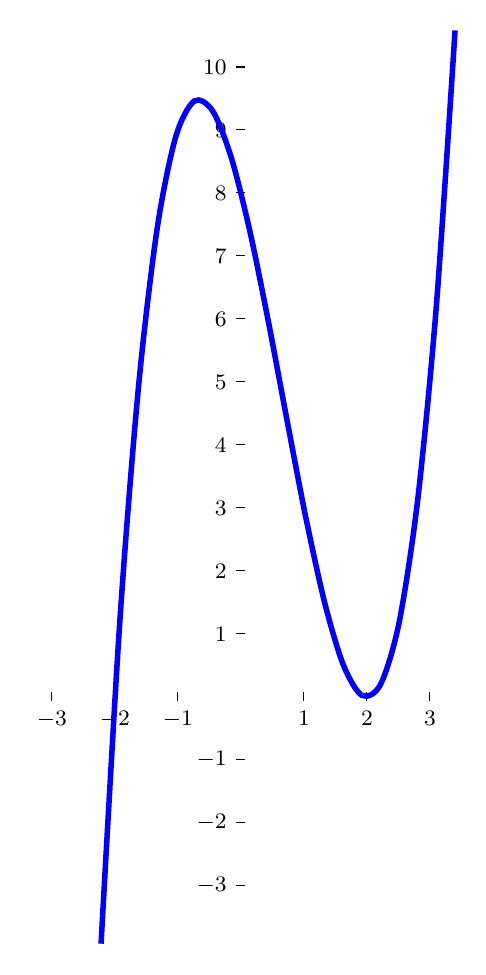
\begin{tikzpicture}[>=latex, scale=0.8]
\koordinate{-3}{4}{-3}{10}
\foreach \x in {-3,...,-1,1,2,...,3}
\draw[shift={(\x,0)}] (0pt,2pt) -- (0pt,-2pt) node[below] {\footnotesize $\x$};
\foreach \y in {-3,...,-1,1,2,...,10}
\draw[shift={(0,\y)}] (2pt,0pt) -- (-2pt,0pt) node[left] {\footnotesize $\y$};
\draw[line width=2.pt,color=blue,smooth,samples=20,domain=-2.22:3.4] plot(\x,{(\x)^3-2*(\x)^2-4*(\x)+8});

\end{tikzpicture}
\end{figure}





%\begin{tikzpicture}
%\draw[help lines, ->] (0,-1) --(0,10);
%\draw[help lines, ->] (-4,0) --(4,0);
%\foreach \x in {-4,-3,-2,-1,0,1,2,3}\draw[shift={(\x,0)},color=black] (0pt,2pt) -- (0pt,-2pt) node[below] %{\footnotesize $\x$};
%\foreach \y in {-1,0,1,2,3,4,5,6,7,8,9,10}\draw[shift={(0,\y)},color=black] (2pt,0pt) -- (-2pt,0pt) node[left] %{\footnotesize $\y$};
%\draw[blue, domain=-2.1:3.3] plot (\x, {(\x)^3-2*((\x)^2)-(4*(\x))+8});
%\end{tikzpicture}
\end{enumerate}
  \end{odgovor}
\end{vaja}



%%%%%%%%%%%%%%%%%%%%%%%%%%%%%%%%%%%%%%%%%%%%%%%%%%%%%%%%%%%%%%%%%%%%%%
% Treba je zapredi datoteko z odgovori

\Closesolutionfile{odgovor}

%%%%%%%%%%%%%%%%%%%%%%%%%%%%%%%%%%%%%%%%%%%%%%%%%%%%%%%%%%%%%%%%%%%%%%
% Odgovori

\section{Odgovori}
\label{sec:polinomi-odgovori}

% Vključimo odgovore.
\input{\datotekaOdgovori}


%%% Local Variables:
%%% mode: latex
%%% TeX-master: "vaje"
%%% End:
